\chapter{Analisi della Compressione e Ricostruzione Storica}
\label{ch:analisi_compressione}
\section{Valutazione della PCA e dell'AE Lineare: il benchmark della linearità}
\label{sec:risultati_pca_linear}

La prima fase di validazione empirica ha avuto come obiettivo la misurazione delle capacità di ricostruzione dei modelli puramente lineari. Come descritto nel Capitolo~\ref{ch:preprocessing}, l'input fornito ai modelli non è costituito dalle serie storiche dei rendimenti originali, bensì dai vettori appiattiti $\mathbf{x} \in \mathbb{R}^{65703}$ rappresentanti la decomposizione di Cholesky delle matrici di correlazione mobili. Di conseguenza, la PCA in questa fase non estrae il classico "fattore di mercato" associato ai titoli (che deriverebbe dall'autodecomposizione dei rendimenti), ma identifica le direzioni di massima varianza nello \emph{spazio delle correlazioni/Cholesky}, tipicamente dominate dalla tendenza sistemica delle correlazioni \emph{pairwise} a variare coralmente nel tempo (il cosiddetto \emph{breathing effect}, o "respiro" del mercato).

Le misurazioni sul \emph{Training Set} hanno confermato rigorosamente il teorema di Bourlard e Kamp (1988): a parità di dimensione del collo di bottiglia $K$, l'Autoencoder Lineare (privo di \emph{bias} e funzioni di attivazione) converge asintoticamente al medesimo Errore Quadratico Medio (MSE) della \emph{Principal Component Analysis} (PCA), con uno scarto relativo inferiore al 20\% a ogni $K$ testato (Tabella~\ref{tab:mse_test_cholesky}). Fissato questo limite, la PCA e il Linear AE stabiliscono il \emph{benchmark} assoluto per la pura compressione lineare dello spazio delle correlazioni: qualsiasi architettura profonda proposta deve dimostrare di poter infrangere tale soglia sfruttando la propria espressività topologica.

\begin{table}[h!]
\centering
\begin{tabular}{lrrrr}
\hline
\textbf{Metodo} & $K=3$ & $K=10$ & $K=20$ & $K=100$ \\
\hline
PCA & $3.56\times10^{-3}$ & $5.55\times10^{-4}$ & $2.73\times10^{-4}$ & $7.39\times10^{-5}$ \\
Linear AE & $4.14\times10^{-3}$ & $6.72\times10^{-4}$ & $3.38\times10^{-4}$ & $8.19\times10^{-5}$ \\
Autoencoder Profondo & $1.70\times10^{-4}$ & $8.45\times10^{-5}$ & $7.19\times10^{-5}$ & $7.34\times10^{-5}$ \\
VAE & --- & --- & $1.55\times10^{-4}$ & --- \\
\hline
\end{tabular}
\caption{Errore quadratico medio (MSE) di ricostruzione sul \emph{Test Set}, dominio Cholesky, al variare della dimensione latente $K$. Il VAE è stato valutato solo a $K=20$ (si veda la nota alla Tabella~\ref{tab:mst_test_cholesky}).}
\label{tab:mse_test_cholesky}
\end{table}

\begin{figure}[h!]
\centering
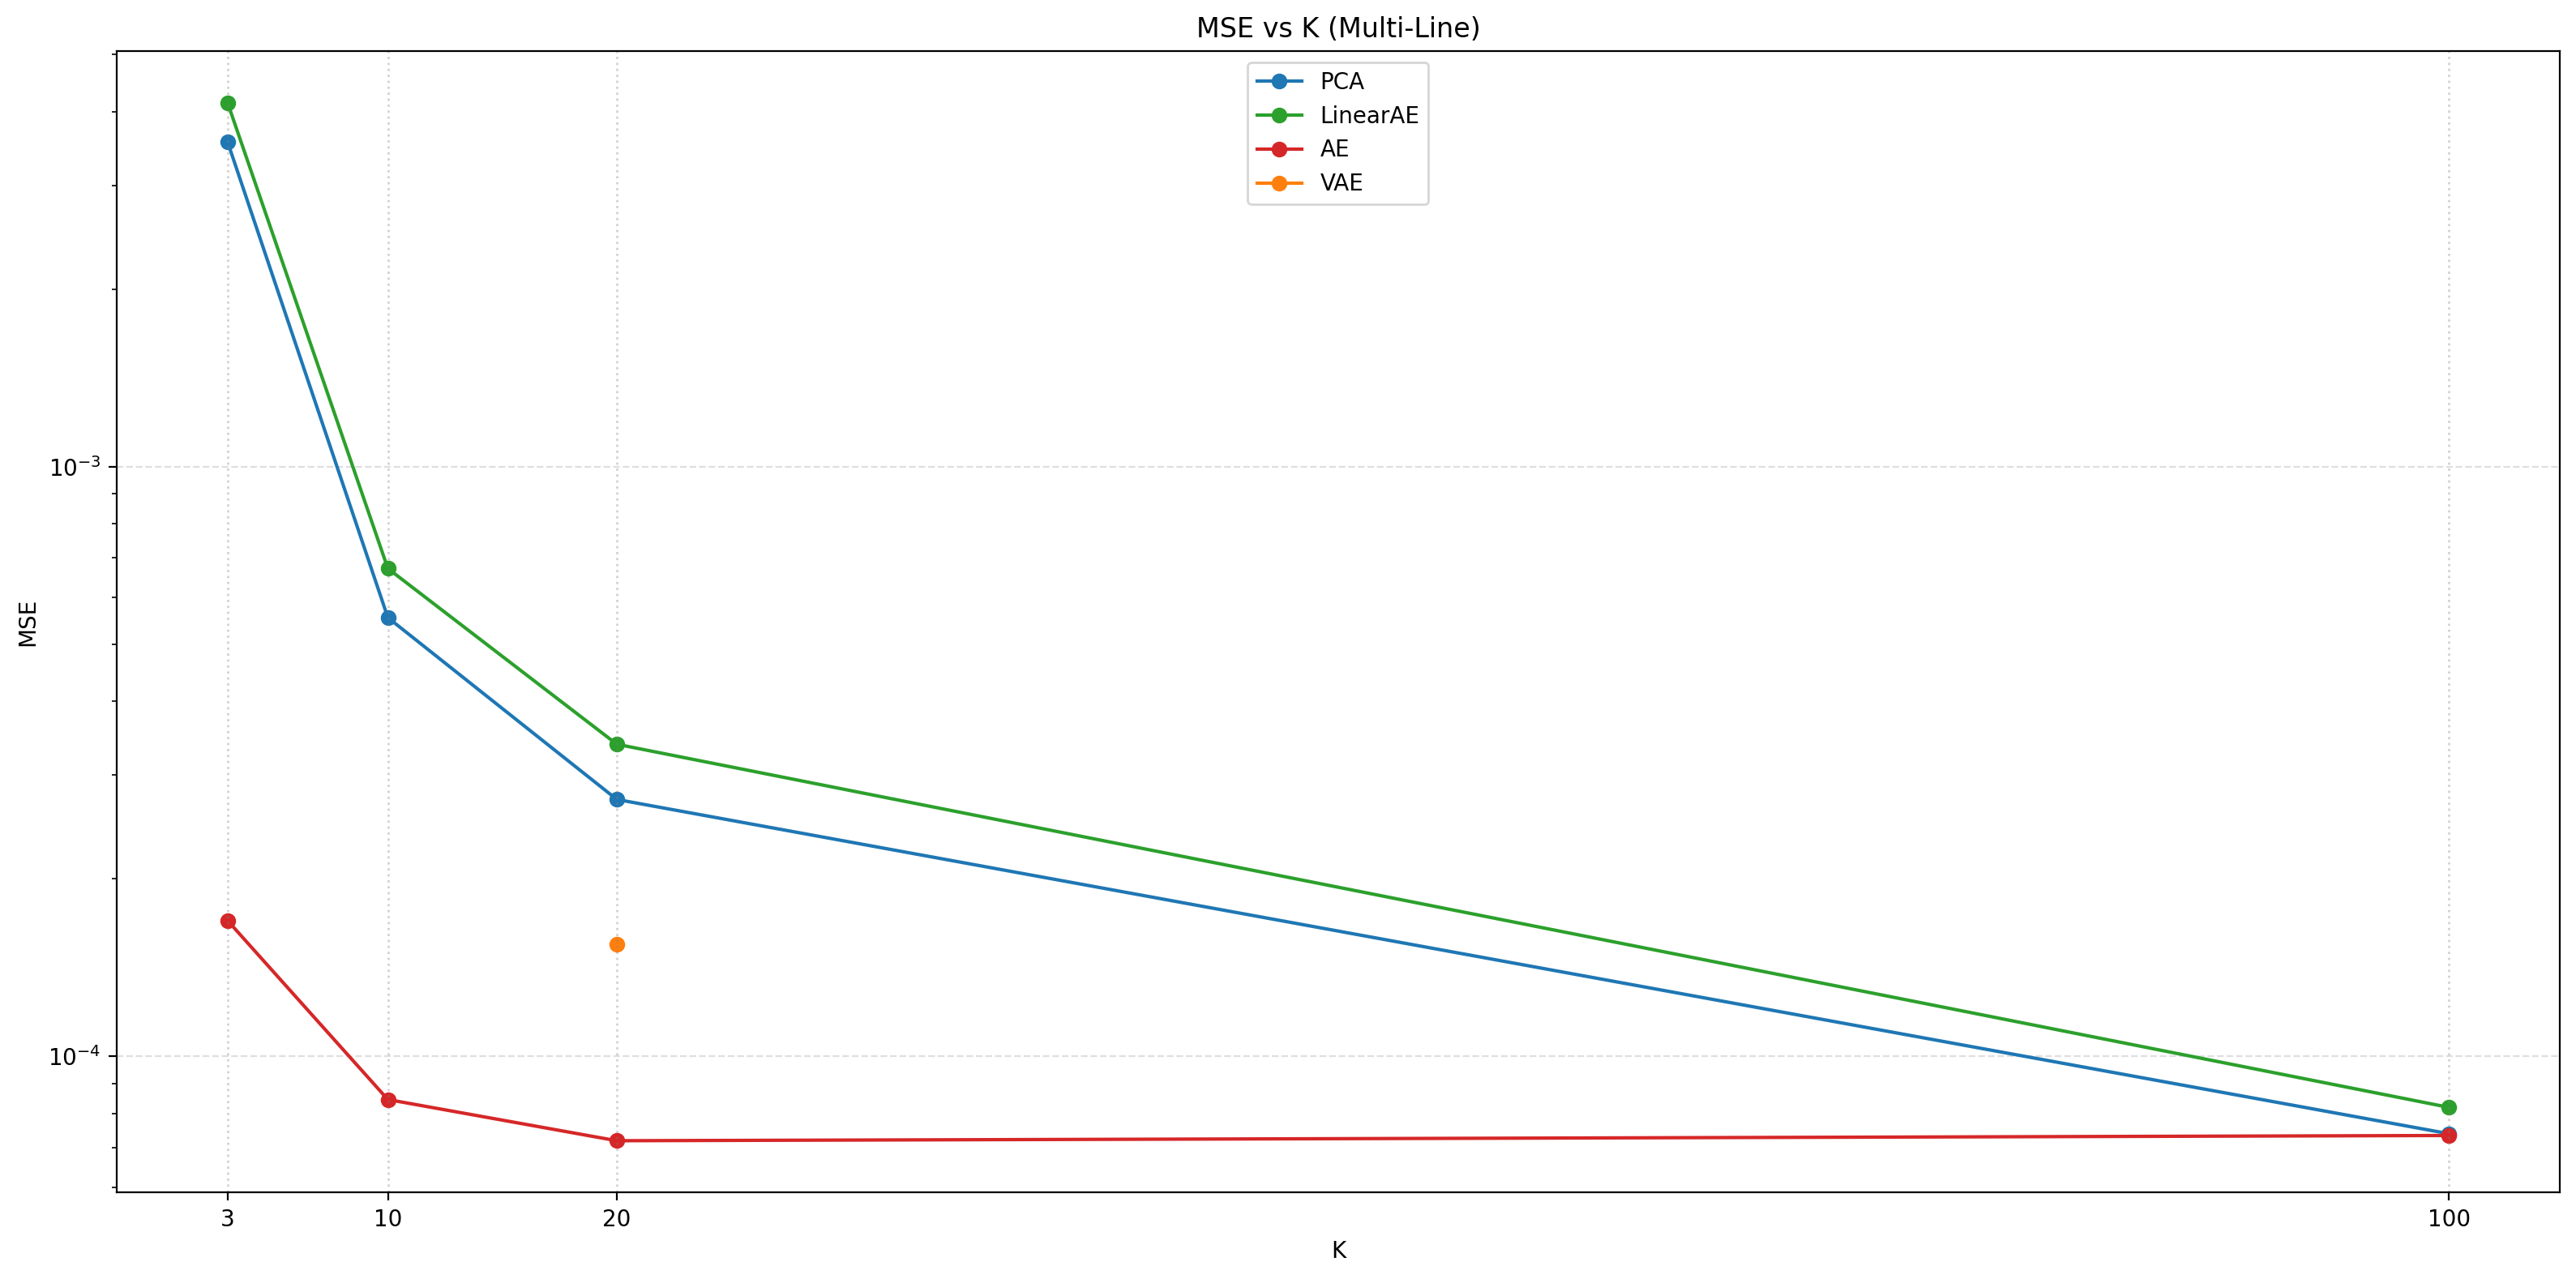
\includegraphics[width=0.75\textwidth]{./Pictures/capitolo7/fig_mse_vs_k.png}
\caption{MSE di ricostruzione sul \emph{Test Set} (dominio Cholesky) in funzione della dimensione latente $K$, per i quattro modelli confrontati (scala logaritmica).}
\label{fig:mse_vs_k}
\end{figure}

Tuttavia, l'analisi dell'errore di ricostruzione sul \emph{Test Set} (Figura~\ref{fig:mse_vs_k}) rivela il limite strutturale di questi approcci: a ogni valore di $K$, sia la PCA sia il Linear AE restano nettamente al di sopra dell'errore dell'Autoencoder Profondo (Sezione~\ref{sec:risultati_ae_vae}). La rigidità dell'iperpiano di proiezione impedisce ai modelli lineari di adattarsi alle complesse interdipendenze non lineari che governano le rotazioni settoriali e le asimmetrie strutturali tra diversi regimi di mercato. La PCA comprime l'informazione in modo algebricamente efficiente, ma restituisce una ricostruzione storicamente "appiattita", faticando a preservare la complessa microstruttura dei veri \emph{stylized facts} finanziari.

\section{Performance di ricostruzione: AE Non-Lineare e VAE}
\label{sec:risultati_ae_vae}

L'introduzione della non-linearità attraverso l'Autoencoder Profondo (Deep AE) ha prodotto un netto superamento del limite imposto dalla PCA, sia sul \emph{Training Set} sia, cosa più rilevante, sul \emph{Test Set} mai visto durante l'addestramento (Tabella~\ref{tab:mse_test_cholesky} e Figura~\ref{fig:mse_vs_k}): a $K=20$, ad esempio, l'MSE di test dell'AE ($7.19\times10^{-5}$) è di quasi quattro volte inferiore a quello della PCA ($2.73\times10^{-4}$). Questo risultato è reso possibile dall'omogeneizzazione statistica introdotta dal campionamento a mescolamento casuale (Capitolo~\ref{ch:preprocessing}): a differenza di quanto osservato nei test preliminari con partizionamento temporale sequenziale (dove il \emph{distribution shift} tra regimi macroeconomici impediva ai modelli non lineari di generalizzare, portandoli persino a essere superati dalla PCA), nella pipeline definitiva l'Autoencoder Profondo non mostra segni di \emph{overfitting}: \emph{Training Loss} e \emph{Validation/Test Loss} rimangono stabilmente allineate su tutto l'arco di $K$ testati.

Il passaggio al Variational Autoencoder (VAE) introduce una dinamica prestazionale più sfumata di quanto una prima intuizione potrebbe suggerire. Il VAE, addestrato nella parametrizzazione Cholesky con la \emph{Reconstruction Loss} basata sulla Divergenza di Jeffreys (Sezione~\ref{sec:setup_vae}), ottiene a $K=20$ un MSE di test pari a $1.55\times10^{-4}$, \textbf{inferiore} sia a quello della PCA ($2.73\times10^{-4}$) sia a quello del Linear AE ($3.38\times10^{-4}$), pur restando superiore a quello dell'Autoencoder Profondo deterministico ($7.19\times10^{-5}$).

\begin{table}[h!]
\centering
\begin{tabular}{lrrrr}
\hline
\textbf{Metrica MST ($K=20$, Test)} & PCA & Linear AE & AE & VAE \\
\hline
\emph{Edge overlap} (\%) & 83.0 & 83.1 & 91.1 & 88.4 \\
\emph{Edge Jaccard} (\%) & 71.2 & 71.4 & 84.0 & 79.4 \\
Distanza $L_1$ distribuzione di grado & 0.081 & 0.084 & 0.068 & 0.076 \\
\emph{Betweenness} \emph{top-10} overlap (\%) & 71.7 & 68.6 & 80.2 & 77.9 \\
\hline
\end{tabular}
\caption{Metriche topologiche di similarità del Minimum Spanning Tree tra matrice originale e ricostruita, dominio Cholesky, $K=20$, \emph{Test Set}. Il VAE non è mai stato confrontato a $K=3$ o $K=100$: si vedano le Osservazioni a fine sezione.}
\label{tab:mst_test_cholesky}
\end{table}

\begin{figure}[h!]
\centering
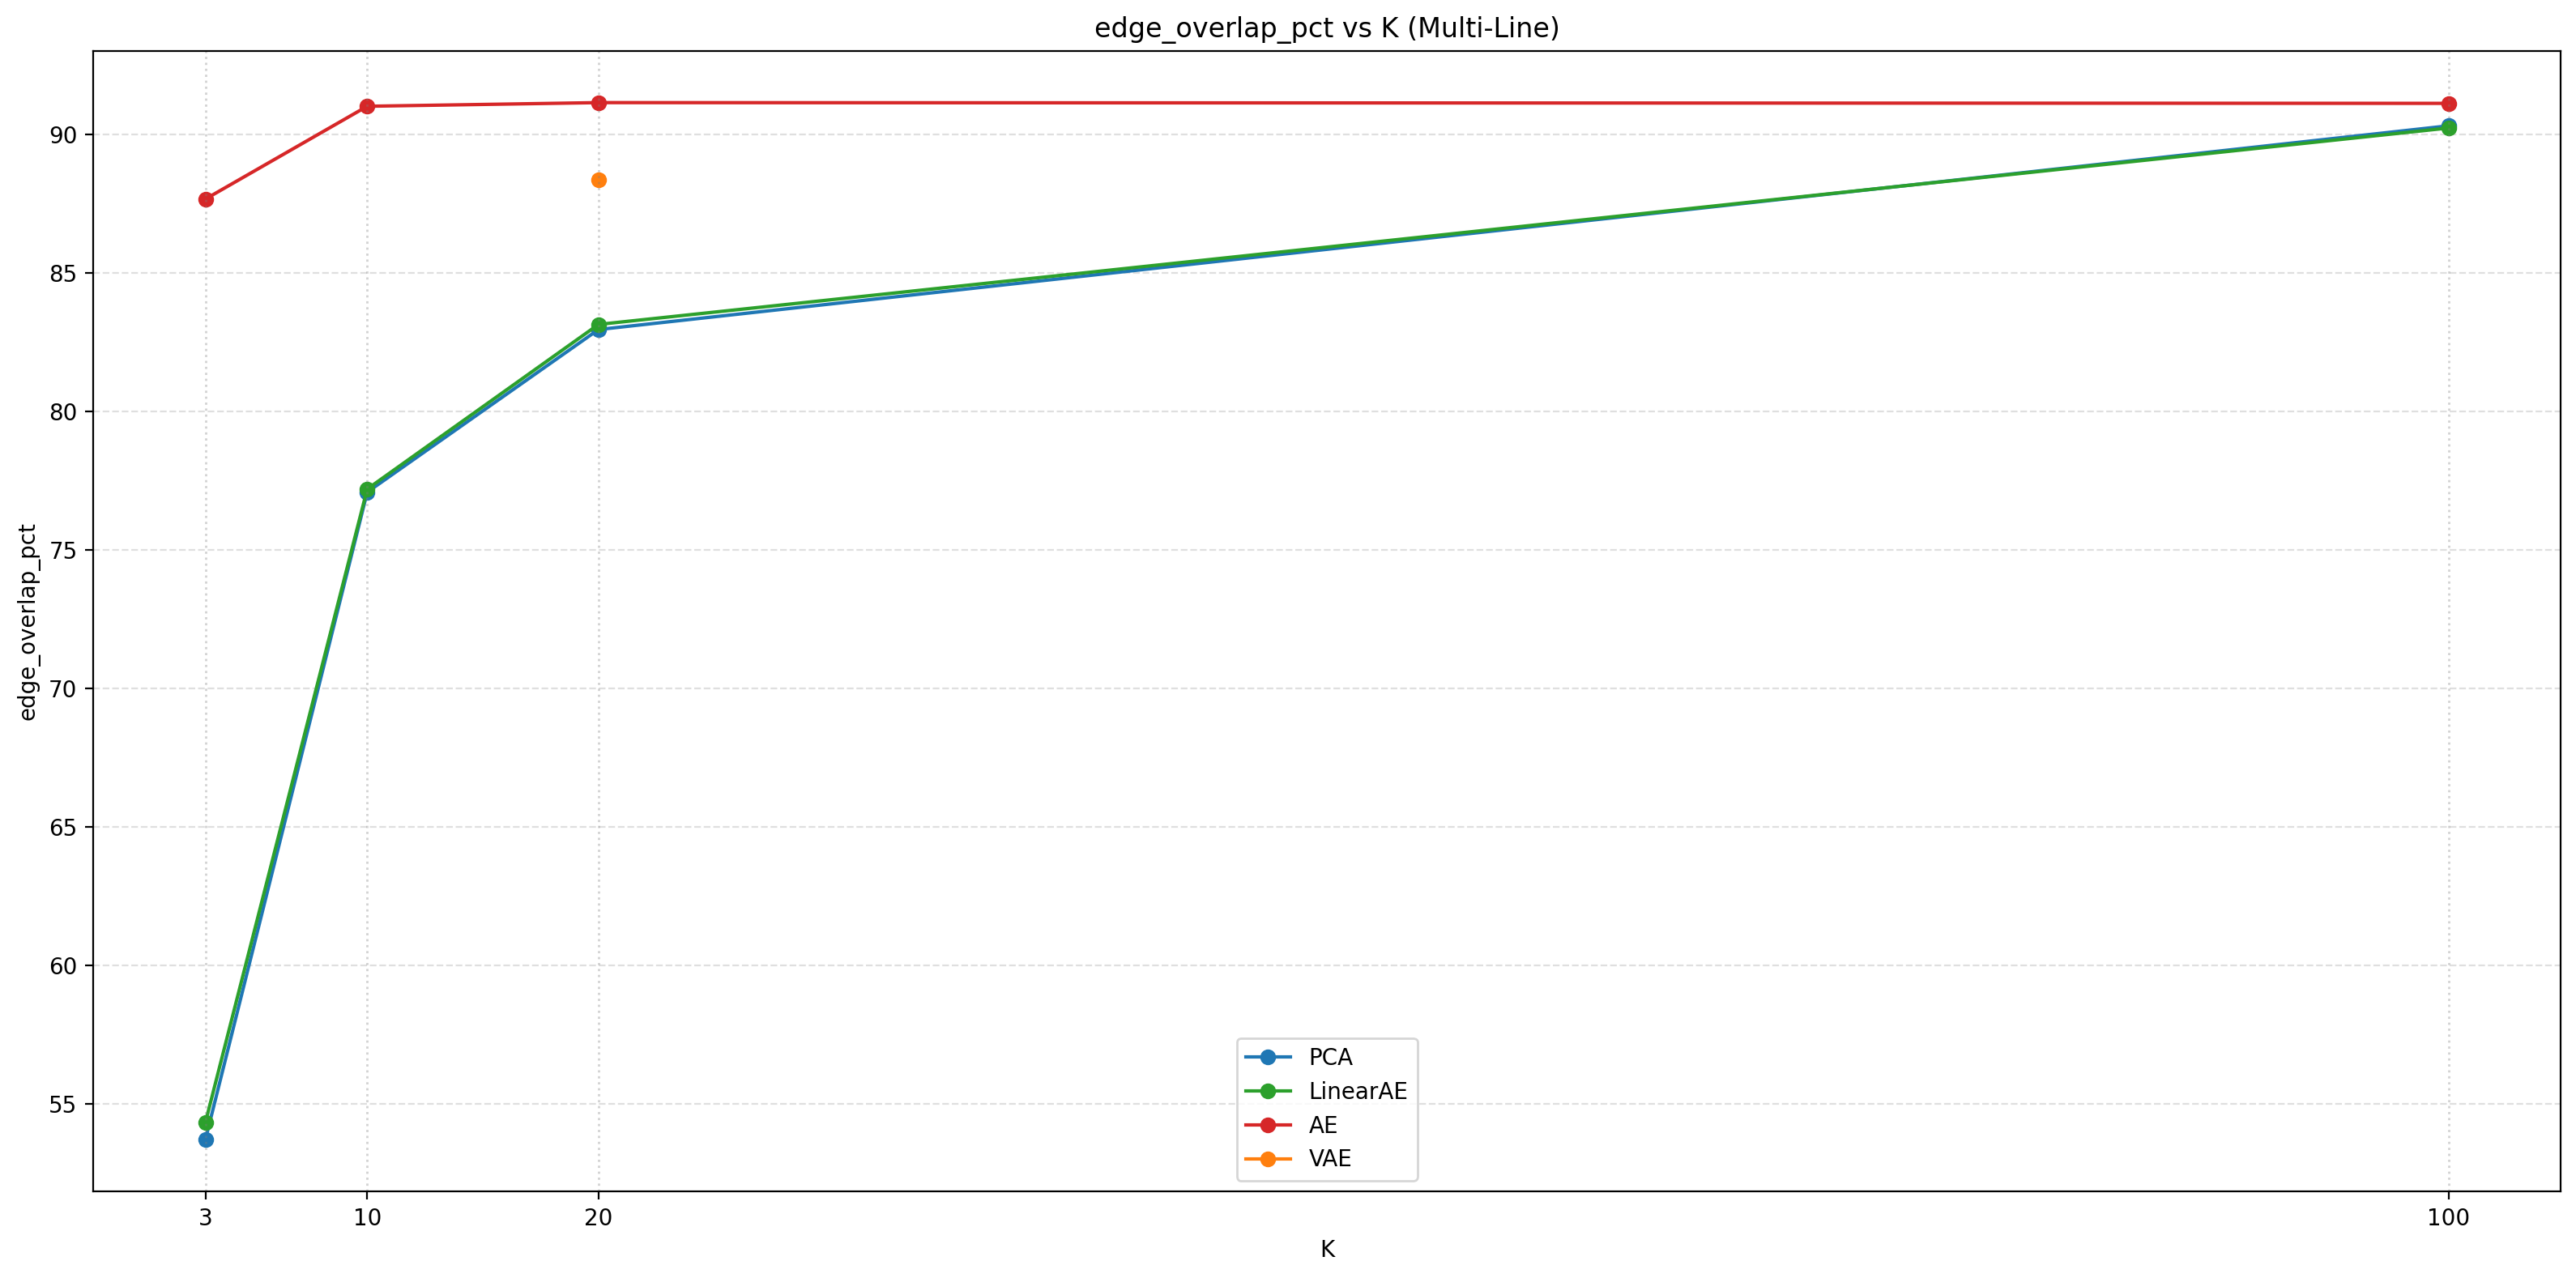
\includegraphics[width=0.75\textwidth]{./Pictures/capitolo7/fig_mst_edge_overlap_vs_k.png}
\caption{Percentuale di archi in comune tra l'MST della matrice originale e quello della matrice ricostruita, dominio Cholesky, \emph{Test Set}, in funzione di $K$.}
\label{fig:mst_edge_overlap_vs_k}
\end{figure}

Le metriche topologiche basate sul Minimum Spanning Tree (Tabella~\ref{tab:mst_test_cholesky} e Figura~\ref{fig:mst_edge_overlap_vs_k}) confermano lo stesso ordinamento: l'Autoencoder Profondo preserva la topologia di rete meglio di tutti gli altri modelli a ogni $K$; il VAE si colloca sistematicamente in posizione intermedia, superando nettamente PCA e Linear AE pur non raggiungendo la fedeltà topologica dell'AE deterministico.

Questo risultato non è casuale, ma la diretta conseguenza della natura della \emph{Reconstruction Loss} impiegata: la loss basata sulla Divergenza di Jeffreys (Sezione~\ref{sec:setup_vae}) pesa esplicitamente l'errore sulla struttura spettrale della matrice di correlazione ricostruita, anziché limitarsi a un errore elemento-per-elemento sui coefficienti del fattore di Cholesky; questa parametrizzazione più informativa, unita alla garanzia strutturale di PSD, riduce significativamente il costo che il vincolo di regolarizzazione $D_{KL}$ impone alla fedeltà di ricostruzione.

\begin{osservazione}
Il confronto a $K=20$ presentato in questa sezione è l'unico punto in cui tutti e quattro i modelli sono stati valutati sullo stesso \emph{Test Set} con la stessa metodologia. Il VAE non è stato sistematicamente confrontato a $K=3$ o $K=100$; inoltre l'errore di ricostruzione del VAE, a differenza degli altri tre modelli, non decresce monotonicamente con $K$ (MSE sul \emph{Training Set}: $6.33\times10^{-5}$ a $K=10$, $8.69\times10^{-5}$ a $K=20$, $1.16\times10^{-4}$ a $K=30$) --- un andamento anomalo, verosimilmente legato alla competizione tra ricostruzione e regolarizzazione KL e al fatto che le run confrontate a $K=10,20,30$ non condividono esattamente gli stessi iperparametri di addestramento (non è quindi un \emph{ablation study} controllato sul solo $K$).
\end{osservazione}

\section{Il trade-off tra compressione esatta e flessibilità generativa}
\label{sec:tradeoff_generazione}

I risultati finora descritti delineano il compromesso fondamentale che giustifica l'adozione delle architetture variazionali in finanza quantitativa. Non si tratta, come i risultati del dominio Cholesky dimostrano, di una dicotomia netta tra "il VAE ricostruisce peggio di tutto" e "il VAE genera scenari realistici": il VAE resta competitivo, e anzi superiore, ai \emph{benchmark} lineari anche in pura ricostruzione. Il compromesso reale è più circoscritto, e riguarda specificamente il confronto tra Autoencoder Profondo deterministico e VAE.

L'Autoencoder Profondo deterministico massimizza l'efficacia della compressione storica (Sezione~\ref{sec:risultati_ae_vae}), ma fallisce totalmente qualora lo si voglia utilizzare come motore di simulazione. Poiché lo spazio latente di un AE classico non è governato da alcuna restrizione probabilistica, i vettori $\mathbf{z}$ si dispongono in modo disaggregato e frammentario, creando vaste regioni di vuoto geometrico (Capitolo~\ref{ch:modelli_generativi}, \S\ref{sec:deep_ae}). Tentare di generare nuovi scenari campionando un vettore casuale da tale spazio e proiettandolo attraverso il \emph{Decoder} produce output privi di coerenza economico-finanziaria. L'AE deterministico è quindi confinato alla pura memorizzazione di un passato statico, per quanto accurata.

Il VAE, pur restando lievemente meno accurato dell'AE nella pura ricostruzione (Tabella~\ref{tab:mse_test_cholesky}), paga questo scarto --- contenuto, e non catastrofico come inizialmente ipotizzato --- in cambio dell'unica proprietà che rende possibile la generazione stocastica: un vincolo di regolarizzazione ($D_{KL}$) che modella uno spazio latente continuo, denso e privo di singolarità, in cui è possibile campionare in modo significativo (Capitolo~\ref{ch:modelli_generativi}, \S\ref{sec:vae}). È proprio questa capacità generativa, resa possibile senza rinunciare in modo sostanziale alla fedeltà di ricostruzione, a motivare la scelta del VAE come modello finale per la generazione di scenari sintetici affrontata nel Capitolo~\ref{ch:generazione_stocastica}, dove la procedura di campionamento effettivamente adottata (un \emph{block-bootstrap} storico nello spazio latente) e la validazione delle matrici generate sui cinque fatti stilizzati del Capitolo~\ref{ch:stylized_facts} vengono presentate in dettaglio.
